\documentclass[../main.text]{subfiles}
\begin{document}

%%find a citation that talks about categorical data in set theoretic terms

Categorical data can be likened to set measurment, where each category is a set
and researchers often want to know how many members each set has and what
intersections are common between sets. It is the latter that is analogous to a
conditional probability, the question of the likelihood of membership in one
set given membership in another. And sometimes there is also a quantative
component involved too. For example, in a study of how NEH funding has changed
over time, there are questions of the likelihoods of different disciplines
being funded (\{d_0,\dots,\d_i}\in \D), and if that is conditioned on
  institutione
  type \{i_0, \dots,\i_n}\in I}, and if either of
those are then conditional on time \{t_0, \dots,t_n} \cite{wired} 
%% this can as easily be 311 data, but I don't have a citation for that
 The most common approach is usually to create a list of frequncies, sometimes of
 sets of one category, such as \D, or a table wherein each cell is a an element
 in the product of two (or more sets), such as \D\cross \I creates a table
 wherein cell one is the frequency of elements that are in both $\d_0$ and
 $\i_0$ \cite{find_pivot_table_citation, set theoreitoc categorical data citation}.

 While a table is encouraged for a small number of variables
 \cite{munznertablesgood}), bar graphs are typically used to display
 differences between subsets such as \d_0,\dots, \d_n \cite{riendly_visualizing_2000,,
   ioannidis_history_2003-1, friendly_brief_2006}. They are somewhat limited to
 showing singular frequencies, in that multiple sets can be shown using
 different colors \cite{semiology} but the bars can not really be used to show
 joint set membership.
 

 \begin{figure}
   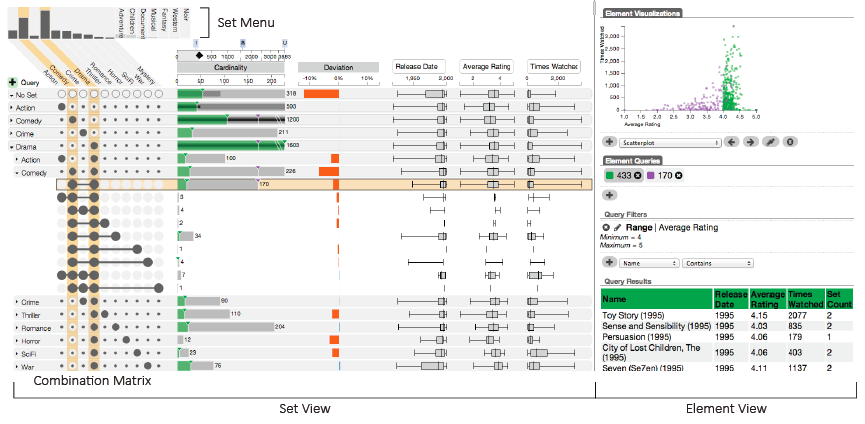
\includegraphics{upsetfig1}
   \caption{UpSet dashboard displaying the relationships amongst movie
     genres. On the left is the set visualiztion; the columns are the sets and
     the rows are the exclusive intersections or aggregates. On the right is
     the element view, and the scatter plot is a comparison of two sets with
     each dot equaling one element in the set.}
   \label{fig:upsetfig1}
 \end{figure}

 
The UpSet tool is designed to display set intersections and the aggregate
information of quantative attributes and set membership.
As shown in \ref{fig:upsetfig4}, the Upset tool provides linked set and element views. The set view provides the intersections and their
aggregates, the frequencies of each set and intersection, and the aggregate
statistics of the associated quantative variables, while the element view shows
selected elements and information about their set membership. The Upset tool
also faciliatates comparison of filtered sets via scatterplot, which acts as a
visualization of the attributes of the data conditioned on membership in the
filtered set.  
 



\end{document}
